\documentclass[12pt]{article}
\usepackage[left=1cm, right=1cm, top=2cm,bottom=1.5cm]{geometry} 

\usepackage[parfill]{parskip}
\usepackage[utf8]{inputenc}
\usepackage[T2A]{fontenc}
\usepackage[russian]{babel}
\usepackage{enumitem}
\usepackage[normalem]{ulem}
\usepackage{amsfonts, amsmath, amsthm, amssymb, mathtools,xcolor}
\usepackage{blkarray}

\usepackage{tabularx}
\usepackage{hhline}

\usepackage{accents}
\usepackage{fancyhdr}
\pagestyle{fancy}
\renewcommand{\headrulewidth}{1.5pt}
\renewcommand{\footrulewidth}{1pt}

\usepackage{graphicx}
\usepackage[figurename=Рис.]{caption}
\usepackage{subcaption}
\usepackage{float}

%%Наименование папки откуда забирать изображения
\graphicspath{ {./images/} }

%%Изменение формата для ввода доказательства
\renewcommand{\proofname}{$\square$  \nopunct}
\renewcommand\qedsymbol{$\blacksquare$}

%%Изменение отступа на таблицах
\addto\captionsrussian{%
	\renewcommand{\proofname}{$\square$ \nopunct}%
}
%% Римские цифры
\newcommand{\RN}[1]{%
	\textup{\uppercase\expandafter{\romannumeral#1}}%
}

%% Для удобства записи
\newcommand{\MR}{\mathbb{R}}
\newcommand{\MC}{\mathbb{C}}
\newcommand{\MQ}{\mathbb{Q}}
\newcommand{\MN}{\mathbb{N}}
\newcommand{\MZ}{\mathbb{Z}}
\newcommand{\MTB}{\mathbb{T}}
\newcommand{\MTI}{\mathbb{I}}
\newcommand{\MI}{\mathrm{I}}
\newcommand{\MCI}{\mathcal{I}}
\newcommand{\MJ}{\mathrm{J}}
\newcommand{\MH}{\mathrm{H}}
\newcommand{\MT}{\mathrm{T}}
\newcommand{\MU}{\mathcal{U}}
\newcommand{\MV}{\mathcal{V}}
\newcommand{\MB}{\mathcal{B}}
\newcommand{\MF}{\mathcal{F}}
\newcommand{\MW}{\mathcal{W}}
\newcommand{\ML}{\mathcal{L}}
\newcommand{\MP}{\mathcal{P}}
\newcommand{\VN}{\varnothing}
\newcommand{\VE}{\varepsilon}
\newcommand{\dx}{\, dx}
\newcommand{\dy}{\, dy}
\newcommand{\dz}{\, dz}
\newcommand{\dd}{\, d}


\theoremstyle{definition}
\newtheorem{defn}{Опр:}
\newtheorem{rem}{Rm:}
\newtheorem{prop}{Утв.}
\newtheorem{exrc}{Упр.}
\newtheorem{problem}{Задача}
\newtheorem{lemma}{Лемма}
\newtheorem{theorem}{Теорема}
\newtheorem{corollary}{Следствие}

\newenvironment{cusdefn}[1]
{\renewcommand\thedefn{#1}\defn}
{\enddefn}

\DeclareRobustCommand{\divby}{%
	\mathrel{\text{\vbox{\baselineskip.65ex\lineskiplimit0pt\hbox{.}\hbox{.}\hbox{.}}}}%
}
\DeclareRobustCommand{\ndivby}{\mkern-1mu\not\mathrel{\mkern4.5mu\divby}\mkern1mu}


%Короткий минус
\DeclareMathSymbol{\SMN}{\mathbin}{AMSa}{"39}
%Длинная шапка
\newcommand{\overbar}[1]{\mkern 1.5mu\overline{\mkern-1.5mu#1\mkern-1.5mu}\mkern 1.5mu}
%Функция знака
\DeclareMathOperator{\sgn}{sgn}

%Функция ранга
\DeclareMathOperator{\rk}{\text{rk}}
\DeclareMathOperator{\diam}{\text{diam}}


%Обозначение константы
\DeclareMathOperator{\const}{\text{const}}

\DeclareMathOperator{\codim}{\text{codim}}

\DeclareMathOperator*{\dsum}{\displaystyle\sum}
\newcommand{\ddsum}[2]{\displaystyle\sum\limits_{#1}^{#2}}

%Интеграл в большом формате
\DeclareMathOperator{\dint}{\displaystyle\int}
\newcommand{\ddint}[2]{\displaystyle\int\limits_{#1}^{#2}}
\newcommand{\ssum}[1]{\displaystyle \sum\limits_{n=1}^{\infty}{#1}_n}

\newcommand{\smallerrel}[1]{\mathrel{\mathpalette\smallerrelaux{#1}}}
\newcommand{\smallerrelaux}[2]{\raisebox{.1ex}{\scalebox{.75}{$#1#2$}}}

\newcommand{\smallin}{\smallerrel{\in}}
\newcommand{\smallnotin}{\smallerrel{\notin}}

\newcommand*{\medcap}{\mathbin{\scalebox{1.25}{\ensuremath{\cap}}}}%
\newcommand*{\medcup}{\mathbin{\scalebox{1.25}{\ensuremath{\cup}}}}%

\makeatletter
\newcommand{\vast}{\bBigg@{3.5}}
\newcommand{\Vast}{\bBigg@{5}}
\makeatother

%Промежуточное значение для sup\inf, поскольку они имеют разную высоту
\newcommand{\newsup}{\mathop{\smash{\mathrm{sup}}}}
\newcommand{\newinf}{\mathop{\mathrm{inf}\vphantom{\mathrm{sup}}}}

%Скалярное произведение
\newcommand{\inner}[2]{\left\langle #1, #2 \right\rangle }
\newcommand{\linsp}[1]{\left\langle #1 \right\rangle }
\newcommand{\linmer}[2]{\left\langle #1 \vert #2\right\rangle }

%Подпись символов снизу
\newcommand{\ubar}[1]{\underaccent{\bar}{#1}}

%% Шапка для букв сверху
\newcommand{\wte}[1]{\widetilde{#1}}
\newcommand{\wht}[1]{\widehat{#1}}
\newcommand{\ovl}[1]{\overline{#1}}

%%Трансформация Фурье
\newcommand{\fourt}[1]{\mathcal{F}\left(#1\right)}
\newcommand{\ifourt}[1]{\mathcal{F}^{-1}\left(#1\right)}

%%Символ вектора
\newcommand{\vecm}[1]{\overrightarrow{#1\,}}

%%Пространстов матриц
\newcommand{\matsq}[1]{\operatorname{Mat}_{#1}}
\newcommand{\mat}[2]{\operatorname{Mat}_{#1, #2}}

%Оператор для действ и мнимых чисел
\DeclareMathOperator{\IM}{\operatorname{Im}}
\DeclareMathOperator{\RE}{\operatorname{Re}}
\DeclareMathOperator{\li}{\operatorname{li}}
\DeclareMathOperator{\GL}{\operatorname{GL}}
\DeclareMathOperator{\SL}{\operatorname{SL}}
\DeclareMathOperator{\Char}{\operatorname{char}}
\DeclareMathOperator\Arg{Arg}

%Делимость чисел
\newcommand{\modn}[3]{#1 \equiv #2 \; (\bmod \; #3)}


%%Взятие в скобки, модули и норму
\newcommand{\parfit}[1]{\left( #1 \right)}
\newcommand{\modfit}[1]{\left| #1 \right|}
\newcommand{\sqparfit}[1]{\left\{ #1 \right\}}
\newcommand{\normfit}[1]{\left\| #1 \right\|}

%%Функция для обозначения равномерной сходимости по множеству
\newcommand{\uconv}[1]{\overset{#1}{\rightrightarrows}}
\newcommand{\uconvm}[2]{\overset{#1}{\underset{#2}{\rightrightarrows}}}


%%Функция для обозначения нижнего и верхнего интегралов
\def\upint{\mathchoice%
	{\mkern13mu\overline{\vphantom{\intop}\mkern7mu}\mkern-20mu}%
	{\mkern7mu\overline{\vphantom{\intop}\mkern7mu}\mkern-14mu}%
	{\mkern7mu\overline{\vphantom{\intop}\mkern7mu}\mkern-14mu}%
	{\mkern7mu\overline{\vphantom{\intop}\mkern7mu}\mkern-14mu}%
	\int}
\def\lowint{\mkern3mu\underline{\vphantom{\intop}\mkern7mu}\mkern-10mu\int}

%%След матрицы
\DeclareMathOperator*{\tr}{tr}

\makeatletter
\renewcommand*\env@matrix[1][*\c@MaxMatrixCols c]{%
	\hskip -\arraycolsep
	\let\@ifnextchar\new@ifnextchar
	\array{#1}}
\makeatother


%% Переопределение функции хи, чтобы выглядела более приятно
\makeatletter
\@ifdefinable\@latex@chi{\let\@latex@chi\chi}
\renewcommand*\chi{{\@latex@chi\smash[t]{\mathstrut}}} % want only bottom half of \mathstrut
\makeatletter

\begin{document}
\lhead{Алгебра-\RN{1}}
\chead{Тимашев Д.А.}
\rhead{Лекция - 14}

\section*{Геометрическая интерпритация поля комплексных чисел}
Пусть $z = x + iy$, изобразим это число в комплексной плоскости. Пусть $r =|z|$ - длина этого вектора, \\ $\varphi$ - угол на который надо повернуть направление $\RE$ оси, чтобы получить направление вектора $z$.
\begin{figure}[H]
	\centering
	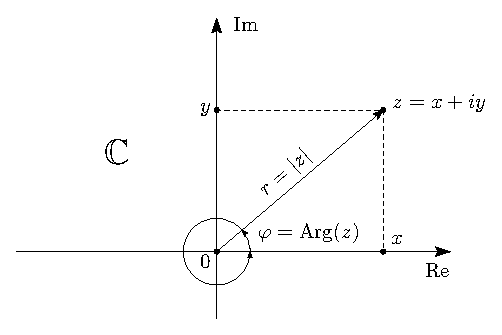
\includegraphics[width=0.35\textwidth]{AL1L14_1.eps}
	\label{AL1L14_1}
	\caption{Геометрическое представление комплексного числа.}
\end{figure}
\begin{defn}
	\uwave{Аргументом} комплексного числа $z \neq 0$: $\Arg{(z)}$ называется угол поворота от положительного направления действительной оси $\RE$ к направлению вектора $z$. Если поворот идёт против часовой стрелки, то этот угол берётся со знаком плюс, если по часовой, то - со знаком минус.
\end{defn}
\begin{rem}
	Знак поворота - это общепринятое соглашение.
\end{rem}

Также заметим, что угол определён неоднозначно, поскольку можно делать полные обороты оси и таких полных оборотов можно сделать сколь угодно много. То есть, аргумент комплексного числа $z$ определен с точностью до прибавления $2\pi k$, где $k \in \MZ \Rightarrow$ аргумент это многозначная функция. 

Иногда бывает удобно выделить среди всех значений аргумента какое-нибудь одно, но в каком-то диапазоне и тогда говорят, что мы выбираем ветвь аргумента.

\begin{defn}
	\uwave{Главной ветвью аргумента} комплексного числа $z \neq 0$: $\arg{(z)}$ называется значение аргумента лежащего в диапазоне $[0,2\pi)$.
\end{defn}
\begin{rem}
	$2\pi$ не включается, для того, чтобы была однозначность.
\end{rem}

Пусть $z = x + iy \in \MC, \, |z| = r, \, \Arg(z) = \varphi$, тогда:
$$
	\left\{
	\begin{matrix}
		x &=& \RE(z) = r{\cdot}\cos{\varphi}\\ 
		y &=& \IM(z) = r{\cdot}\sin{\varphi}
	\end{matrix}
	\right. \Rightarrow z = r{\cdot}(\cos{\varphi} + i\sin{\varphi})
$$
\begin{defn}
	Запись комплексного числа в виде:
	$$
		z = r{\cdot}(\cos{\varphi} + i\sin{\varphi}) = |z|{\cdot}(\cos{\varphi} + i\sin{\varphi})
	$$
	называется \uwave{тригонометрической формой записи комплексного числа}.
\end{defn}
\textbf{\uline{Обозначение}}: $e^{i \varphi} = \cos{\varphi} + i\sin{\varphi}$, (\textbf{формула Эйлера}).
\begin{rem}
	Подчеркнем, что это лишь обозначение. В анализе эту формулу можно доказать.
\end{rem}
\begin{defn}
	Запись комплексного числа в виде:
	$$
		z = r{\cdot}e^{i\varphi} = |z|{\cdot}e^{i\varphi}
	$$
	называется \uwave{экспоненциальной формой записи комплексного числа}.
\end{defn}

\subsection*{Свойства записи комплексных чисел}
\begin{prop}\hfill
	\begin{enumerate}[label=\arabic*)]
		\item $\forall z,w \in \MC,\, |z{\cdot}w| = |z|{\cdot}|w|, \, \Arg{(z{\cdot}w)} = \Arg(z) + \Arg(w)$;
		\item $\forall z \in \MC, \, |\ovl{z}| = |z|, \, \Arg(\ovl{z}) = -\Arg(z)$;
		\item $\forall z \in \MC, \, z = r{\cdot}(\cos{\varphi} + i\sin{\varphi}) \Rightarrow z^n = r^n{\cdot}(\cos(n\varphi) + i\sin(n\varphi)), \, \forall n \in \MZ$, (\textbf{формула Муавра});
		\item $\forall z,w \in \MC,\, \left|\dfrac{w}{z}\right| = \dfrac{|w|}{|z|}, \, \Arg\left(\dfrac{w}{z}\right) = \Arg(w) - \Arg(z)$;
	\end{enumerate}
\end{prop}
\begin{proof}\hfill
	\begin{enumerate}[label=\arabic*)]
		\item Пусть $z = r{\cdot}(\cos{\varphi} + i\sin{\varphi})$ и $w = s{\cdot}(\cos{\psi} + i\sin{\psi})$, перемножим их:
		$$
			z{\cdot}w = r{\cdot}s{\cdot}(\cos{\varphi} + i\sin{\varphi}){\cdot}(\cos{\psi} + i\sin{\psi}) =
		$$
		$$
			= r{\cdot}s{\cdot}(\cos{\varphi}{\cdot}\cos{\psi} - \sin{\varphi}{\cdot}\sin{\psi} + i(\sin{\varphi}{\cdot}\cos{\psi} + \cos{\varphi}{\cdot}\sin{\psi})) = r{\cdot}s{\cdot}(\cos{(\varphi + \psi) + i\sin{(\varphi + \psi)}})\Rightarrow
		$$
		$$
			\Rightarrow z{\cdot}w = r{\cdot}s{\cdot}(\cos{(\varphi + \psi) + i\sin{(\varphi + \psi)}})\Rightarrow |z{\cdot}w| = r{\cdot}s,\, \Arg(z{\cdot}w) = \varphi + \psi = \Arg(z) + \Arg(w)
		$$
		Перепишем это в экспоненциальной форме:
		$$
			z = re^{i\varphi}, \, w = se^{i\psi} \Rightarrow z{\cdot}w = r{\cdot}s{\cdot}e^{i\varphi}{\cdot}e^{i\psi} = r{\cdot}s{\cdot}e^{i(\varphi + \psi)}
		$$
		Таким образом, в этой форме это удобнее запомнить;
		\item Это видно сразу из геометрических соображений: соответствующий вектор получается отражением относительно оси абсцисс (действительной оси) и его длина не меняется, а аргумент меняет направление, поскольку угол поворота тот же самый, но меняет направление.
		\begin{figure}[H]
			\centering
			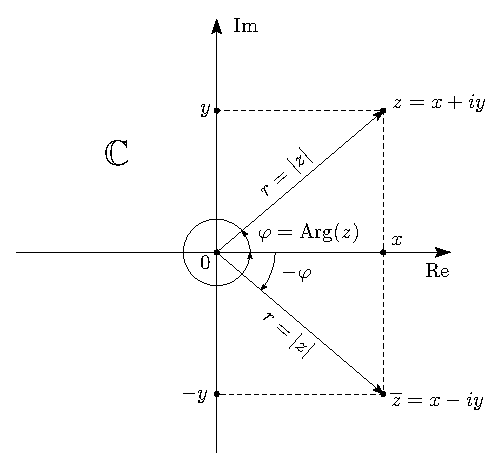
\includegraphics[width=0.4\textwidth]{AL1L14_2.eps}
			\label{AL1L14_2}
			\caption{Модуль и аргумент для сопряженного числа.}
		\end{figure}
		Если $z = x + iy$, то $\ovl{z} = x - iy$, следовательно: 
		$$
			|z| = \sqrt{x^2 + y^2} = |\ovl{z}|
		$$
		$$
			\left\{
			\begin{matrix}
				x &=& \RE(\ovl{z}) = r{\cdot}\cos{\varphi} = r{\cdot}\cos(-\varphi)\\ 
				-y &=& \IM(\ovl{z}) = -r{\cdot}\sin{\varphi} = r{\cdot}\sin(-\varphi)
			\end{matrix}
			\right. \Rightarrow \Arg(\ovl{z}) = -\varphi = -\Arg(z)
		$$
		\item Пусть $n > 0$, тогда по индукции из пункта $1)$:
		$$
			z^n = \underbrace{z{\cdot}\dotsc{\cdot}z}_{n} \Rightarrow |z^n| = |z{\cdot}\dotsc{\cdot}z| = |z|{\cdot}\dotsc{\cdot}|z| = r{\cdot}\dotsc{\cdot}r = r^n
		$$
		$$
			\Arg(z^n) = \Arg(z) + \dotsc + \Arg(z) = \underbrace{\varphi + \dotsc + \varphi}_{n} = n{\cdot}\varphi
		$$
		Пусть $n = 0$, тогда:  $z^0 = 1, \, |1| = 1 = r^0, \, \Arg(1) = 0 = 0{\cdot}\varphi$, поскольку единица это число на действительной оси на положительном направлении, её угол наклона к оси абсции равен нулю.
		
		Пусть $n = -1$, тогда:
		$$
			z^{-1} = \dfrac{\ovl{z}}{|z|^2} = \dfrac{r(\cos(-\varphi) + i\sin(-\varphi))}{r^2} = r^{-1}{\cdot}(\cos(-\varphi) + i\sin(-\varphi))
		$$
		Пусть $n < 0$, тогда по пункту доказательству для $n>0$ будет верно:
		$$
			z^n = (z^{-1})^{|n|} = \left[r^{-1}{\cdot}(\cos(-\varphi) + i\sin(-\varphi))\right]^{|n|} = (r^{-1})^{|n|}{\cdot}(\cos(-|n|{\cdot}\varphi) + i\sin(-|n|{\cdot}\varphi)) = 
		$$
		$$
			= r^n{\cdot}(\cos(n\varphi) + i\sin(n\varphi))
		$$
		\item Это следует из $1)$ и формулы Муавра для $n=-1$:
		$$
			\dfrac{w}{z} = w{\cdot}z^{-1} \Rightarrow \left|\dfrac{w}{z}\right| = | w{\cdot}z^{-1}| = |w|{\cdot}|z^{-1}| = |w|{\cdot}|z|^{-1} = \dfrac{|w|}{|z|}
		$$
		$$
			\Arg\left(\dfrac{w}{z}\right) = \Arg\left(w{\cdot}z^{-1}\right) = \Arg(w) + \Arg(z^{-1}) = \Arg(w) - \Arg(z)
		$$
	\end{enumerate}
\end{proof}

\textbf{Геометрический смысл операции умножения или деления на фиксированное комплексное число}: весь смысл заключается в свойствах $1)$ и $4)$, когда умножаем на $z \in \MC$, то модуль числа умножается на $|z|$ (то есть происходит растяжение или сжатие - гомотетия), а к аргументу прибавляется $\Arg(z)$ (то есть происходит поворот) $\Rightarrow$ умножение/деление на $z \in \MC$ это поворотная гомотетия.

Подводя итоги, можем определить \textbf{геометрический смысл}:
\begin{enumerate}[label=\arabic*)]
	\item \textbf{$+/-$ комплексного числа}: как параллельный перенос на комплексной плоскости;
	\item \textbf{$\cdot/\div$ комплексного числа}: как поворотную гомотетияю;
\end{enumerate}

\subsection*{Применение формулы Муавра}
Одним из очевидных применений формулы Муавра является быстрый расчет $\cos(nx)$ и $\sin(nx)$, для этого нужно раскрыть скобки в биноме соответствующей степени $n$:
$$
	(\cos(x) + i\sin(x))^5 = \cos(5x) + i\sin(5x) 	\Rightarrow (\cos(x) + i\sin(x))^5 = 
$$
$$
	=\cos^5(x) + 5i\cos^4(x)\sin(x) - 10\cos^3(x)\sin^2(x) - 10i\cos^2(x)\sin^3(x) + 5\cos(x) \sin^4(x) + i\sin^5(x)
$$
$$
	 \Rightarrow \cos(5x) = \cos^5(x) - 10\cos^3(x)\sin^2(x) + 5\cos(x)\sin^4(x)
$$
$$
	\Rightarrow \sin(5x) = 5\cos^4(x)\sin(x) - 10 \cos^2(x)\sin^3(x) + \sin^5(x)
$$


\section*{Извлечение корней в $\MC$}
Мы расширяли поле $\MR$ до $\MC$ для того, чтобы была возможность извлекать квадратные корни из отрицательных действительных чисел. Оказывается, что в поле $\MC$ можно делать больше - извлекать корни любой степени из любых комплексных чисел. Извлечение корня это решение уравнений вида:
$$
	w^n = z \Leftrightarrow \sqrt[n]{z} = w
$$
Наша задача - найти все $w$. Запишем это уравнение в тригонометрической форме:
$$
	\begin{cases}
		z = r{\cdot}(\cos\varphi + i \sin \varphi)\\
		w = s{\cdot}(\cos\psi + i \sin\psi)
	\end{cases} \Rightarrow
	w^n = z \Leftrightarrow 
	\begin{cases}
		s^n = r\\
		n\psi = \varphi + 2\pi k, k \in \MZ
	\end{cases}
$$
где аргумент $w^n$ должен быть равен аргументу $z$, но поскольку аргумент это многозначная функция, то значение $n\psi$ должно быть равно одному из значений  аргумента $z$: не обязательно значению $\varphi$, например, может отличаться от $\varphi$ на целое кратное полного оборота. Тогда, поскольку $r,s > 0$, то:
$$
	\begin{cases}
		s^n = r\\
		n\psi = \varphi + 2\pi k, k \in \MZ
	\end{cases} \Leftrightarrow
	\begin{cases}
		s = \sqrt[n]{r}\\
		\psi = \dfrac{\varphi}{n} + \dfrac{2\pi k}{n}, k \in \MZ
	\end{cases}
$$
Заметим, что $k \in \MZ$, но при этом аргументы будут повторяться по модулю $2\pi$ с периодом $n \Rightarrow$ значения аргумента будут различными, если, например, $k = \overline{0, n-1}$, то есть все остатки при делении на $n$.

\begin{prop}
	$\forall z \in \MC, \, z \neq 0$, уравнение $w^n = z$ имеет $n$ различных решений $w_0, \dotsc, w_{n-1} \in \MC$:
	$$
		|w_k| = \sqrt[n]{|z|}, \, \arg(w_k) = \dfrac{\arg(z)}{n} + \dfrac{2\pi k}{n}, \, k = \overline{0,n-1}
	$$
	$$
		w_k = \sqrt[n]{r}{\cdot}\left(\cos\left(\tfrac{\varphi}{n} + \tfrac{2\pi k}{n}\right) + i \sin\left(\tfrac{\varphi}{n} + \tfrac{2\pi k}{n}\right) \right), \, k = \overline{0,n-1}
	$$
\end{prop}
\begin{rem}
	Заметим, что здесь получится именно главная ветвь аргумента, поскольку если $\arg(z) \in [0,2\pi)$, то тогда $\tfrac{\arg(z)}{n} \in \left[0,\tfrac{2\pi}{n}\right) \Rightarrow \arg(w_k)= \tfrac{\arg(z)}{n} + \tfrac{2\pi k}{n} \in [0, 2\pi)$, так как $0 \leq k \leq n-1$. 
\end{rem}
\subsection*{Геометрическая интерпритация}
\begin{figure}[H]
	\centering
	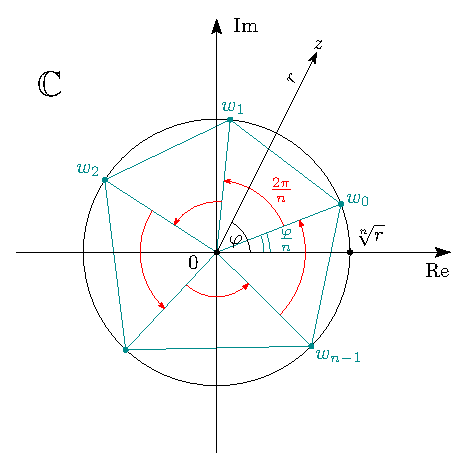
\includegraphics[width=0.4\textwidth]{AL1L14_3.eps}
	\label{AL1L14_3}
	\caption{Геометрическая интерпритация извлечения корней в $\MC$.}
\end{figure}

Пусть есть какое-то число $z$, у него есть модуль равный $r$ и аргумент $\varphi$. Корни $n$-ой степени из числа $z$ имеют одинаковую длину $\sqrt[n]{r} \Rightarrow$ расположены на окружности радиуса $\sqrt[n]{r}$ с центром в начале координат. Число $w_0$ имеет аргумент $\tfrac{\varphi}{n}$, остальные числа также расположены на окружности и каждое следующее число получается прибавлением $\tfrac{2\pi}{n}$ к аргументу предыдущего числа. Последним числом будет $w_{n-1}$, а следующее снова будет $w_0$. 

В результате, все корни находятся в вершинах правильного $n$-угольника, вписаного в окружность радиуса $\sqrt[n]{r}$ с центром в точке $0$ и одна из вершин имеет угол $\tfrac{\varphi}{n}$ по отношению к оси абсцисс, остальные получаются поворотом на $\tfrac{2\pi}{n}$.

\subsection*{Корни степени $n$ из единицы}
Пусть $\VE_0 = 1, \VE_1, \VE_2, \dotsc, \VE_{n-1}$ - корни $n$-ой степени из $1$, то есть решения уравнения: $z^n = 1$. Всего таких корней $n$ штук по утверждению выше. Рассмотрим $k$-ый корень:
$$
	\VE_k = \sqrt[n]{1}{\cdot}\left(\cos\left(\tfrac{0}{n} + \tfrac{2\pi k}{n}\right) + i \sin\left(\tfrac{0}{n} + \tfrac{2\pi k}{n}\right) \right) = \cos\left(\tfrac{2\pi k}{n}\right) + i\sin\left(\tfrac{2\pi k}{n}\right), \, \forall k =\overline{0, n-1}
$$
$$
	|\VE_k| = 1, \, \arg(\VE_k) = \dfrac{2\pi k}{n}, \, \forall k =\overline{0, n-1}
$$
Используя формулу Эйлера, мы можем переписать $k$-ый корни степени $n$ из единицы в следующем виде:
$$
	\VE_k = e^{\tfrac{2\pi k i}{n}}, \, \forall k =\overline{0, n-1}
$$
\begin{figure}[H]
	\centering
	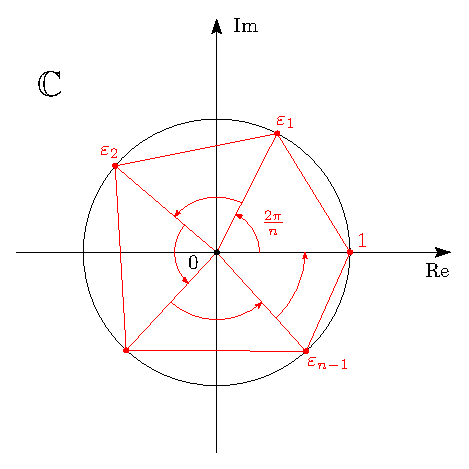
\includegraphics[width=0.4\textwidth]{AL1L14_4.eps}
	\label{AL1L14_4}
	\caption{Единичные корни в комплексной плоскости.}
\end{figure}
Геометрически, корни $n$-ой степени из $1$ расположены в вершинах правильного $n$-угольника, вписанного в единичную окружность на комплексной плоскости, начиная с вершины в точке единицы.
\newpage
\begin{prop}
	\textbf{Свойства корней $n$-ой степени из единицы}
	\begin{enumerate}[label=\arabic*)]
		\item Пусть $w_k$ - корни $n$-ой степени из $z \in \MC$, тогда: $w_k{\cdot}\VE_l = w_{k + l (\bmod n)}$;
		\item $\VE_k{\cdot}\VE_l = \VE_{k + l (\bmod n)}$;
		\item $\VE_k^{-1} = \ovl{\VE_k} = \VE_{-k} = \VE_{n-k}$;
	\end{enumerate}
\end{prop}
\begin{proof}\hfill
	\begin{enumerate}[label=\arabic*)]
		\item По утверждениям выше:
		$$
			|w_k| = \sqrt[n]{r}, \, \arg(w_k) = \dfrac{\arg(z)}{n} + \dfrac{2\pi k}{n}, \, k = \overline{0,n-1} \Rightarrow
		$$
		$$
			\Rightarrow |w_k{\cdot}\VE_l| = |w_k|{\cdot}|\VE_1| = |w_k|{\cdot}1 = |w_k|, \, \arg(w_k{\cdot}\VE_l) = \arg(w_k) + \arg(\VE_l) = 
		$$
		$$
			= \dfrac{\arg(z)}{n} + \dfrac{2\pi k}{n} + \dfrac{2\pi l}{n} = \dfrac{\arg(z)}{n} + \dfrac{2\pi (k + l)}{n} = \dfrac{\arg(z)}{n} + \dfrac{2\pi (k + l) \bmod m}{n} = \arg(w_{k + l(\bmod{m})})
		$$
		\item Применяя свойство $1)$ к $\VE_k$ получаем требуемое;
		\item По свойствам записи комплексных чисел:
		$$
			\VE_k^{-1} = \dfrac{\ovl{\VE_k}}{|\VE_k|^2} = \dfrac{\ovl{\VE_k}}{1^2} = \ovl{\VE_k},\, |\VE_k| = |\ovl{\VE_k}| = 1
		$$
		$$	
			\arg(\ovl{\VE_k}) = - \arg(\VE_k) = - \dfrac{2\pi k}{n} = 2\pi - \dfrac{2\pi k}{n} = \dfrac{2\pi (n -k)}{n} = \arg(\VE_{-k}) = \arg(\VE_{n-k})
		$$
	\end{enumerate}
\end{proof}
\begin{rem}
	Свойство $1)$ сразу дает следующий факт: если мы знаем какой-нибудь $w_k$ - один из корней $n$-ой степени из числа $z$ и если мы знаем все корни $n$-ой степени из единицы, то умножая $w_k$ на всевозможные корни степени $n$ из единицы мы получим все остальные корни степени $n$ из числа $z$, потому что $\VE_k$ соответствуют кратным поворотам на угол $\tfrac{2\pi}{n}$.
\end{rem}

Свойства $2)$ и $3)$ говорят, что множество корней из единицы при фиксированном $n$ замкнуты относительно умножения и взятия обратного элемента. Введём обозначение:
$$
	\mathbb{U}_n = \{1, \VE_1,\dotsc, \VE_{n-1}\}
$$
Тогда $\mathbb{U}_n$ - будет подгруппой в группе $(\MC^{\times}, \cdot)$ - мультипликативной группе комплексных чисел.
\begin{exrc}
	Доказать, что существует изоморфизм $\mathbb{U}_n \simeq \MZ_n$ к аддитивной группе вычетов по модулю $n$.
\end{exrc}
\newpage
\subsection*{Первообразные корни из единицы}
\begin{defn}
	\uwave{Первообразный корень степени $n$ из единицы} - это корень степени $n$ из единицы, не являющийся корнем из единицы никакой меньшей степени $m < n$.
\end{defn}
\begin{rem}
	Любой корень из $1$ является первообразным для какой-то степени $n$.
\end{rem}

\textbf{Пример}: при $n=6$ первообразными корнями будут $\VE_1$ и $\VE_5$:
$$
	\VE^m_k = \left(\cos\left(\tfrac{2\pi k}{6}\right) + i\sin\left(\tfrac{2\pi k}{6}\right)   \right)^m = \cos\left(\tfrac{2\pi km}{6}\right) + i\sin\left(\tfrac{2\pi k m}{6}\right) = \cos(2\pi l) + i\sin(2\pi l), \, m < 6, \, l \in \MN \Rightarrow
$$
$$
	\Rightarrow \dfrac{2 \pi km}{6} = 2\pi l \Leftrightarrow km = 6l \Rightarrow 
	\begin{cases}
		k = 0, m = 1, l = 0\\
		k = 1, m = 6, l = 1\\
		k = 2, m = 3, l = 1\\
		k = 3, m = 2, l = 1\\
		k = 4, m = 3, l = 2\\
		k = 5, m = 6, l = 5
	\end{cases}
$$

\begin{prop}
	Число $\VE_k$ является первообразным корнем степени $n$ из единицы $\Leftrightarrow k$ взаимно просто с $n$, или по-другому: $(k,n) =1$. В частности, первообразные корни существуют для любого $n$.
\end{prop}
\begin{proof}
	Возьмем $\VE_k$ и возведем его в степень $m$:
	$$
		(\VE_k)^m = \VE_{km} = \cos\left(\tfrac{2\pi km}{n}\right) + i\sin\left(\tfrac{2\pi km}{n}\right) = 1\Leftrightarrow \dfrac{km}{n} \in \MZ \Leftrightarrow km \divby n
	$$
	
	$(\Leftarrow)$ Пусть $k$ взаимно просто с $n$, тогда:
	$$
		km \divby n, \, (k,n) = 1 \Rightarrow m \divby n 
	$$
	Следовательно, наименьшее $m$ делящееся на $n$ это $n \Rightarrow  \VE_k$ - первообразный корень степени $n$ из $1$. 
	
	$(\Rightarrow)$ (\uline{От противного}) Пусть $(k,n) = d > 1$, тогда $k = d{\cdot}l, \, n = d{\cdot}m$, тогда:
	$$
		k{\cdot}m = d{\cdot}l{\cdot}m = l{\cdot}n \divby n \Rightarrow (\VE_k)^m = 1, \, m < n
	$$
	Тогда $\VE_k$ не является первообразным корнем степени $n$ из $1 \Rightarrow$ противоречие.
\end{proof}

\begin{prop}
	Если $\VE_k$ - первообразный корень степени $n$, то $\forall \VE_s$ степени $n, \, \exists\,  m \in \MN \colon \VE_s = \VE_k^m$.
\end{prop}
\begin{proof}
	Пусть $\VE_k$ - первообразный корень $\Rightarrow \VE_k, \VE_k^2, \dotsc, \VE_k^{n}$ - попарно различны. Если $\VE_k^p = \VE_k^l, \, l < p$, тогда:
	$$
		\VE_k^l(\VE_k^{p-l} - 1) = 0, \, \VE_k^{l} \neq 0 \Rightarrow \VE_{k}^{p-1} = 1
	$$
	Получаем противоречие с первообразностью, так как $1 \leq p, l \leq n \Rightarrow p - l<n \Rightarrow \VE_{k}^{p-1} \neq 1$. Тогда, среди всех степеней: $\VE_k, \VE_k^2, \dotsc, \VE_k^{n}$ должны встретится все корни: $\VE_0, \VE_1, \dotsc, \VE_{n-1}$.
\end{proof}

\newpage
\textbf{Пример}: $z^{12} = 1 \Rightarrow$ корни $\VE_0 = 1, \dotsc, \VE_{11}$. Найти первообразные корни.

\begin{figure}[H]
	\centering
	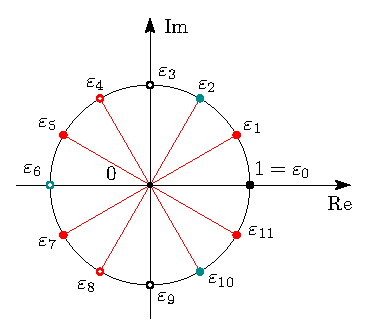
\includegraphics[width=0.5\textwidth]{AL1L14_5.eps}
	\label{AL1L14_5}
	\caption{Единичные корни при $n=12$.}
\end{figure}

Первообразными корнями из $1$ степени $12$ являются: $\VE_1, \, \VE_5, \, \VE_7, \, \VE_{11}$ - отмечены красным.

Первообразными корнями из $1$ степени $6$ являются: $\VE_2, \, \VE_{10}$ - отмечены зеленым.

Первообразными корнями из $1$ степени $4$ являются: $\VE_3, \, \VE_{9}$ - отмечены черным выколотым.

Первообразными корнями из $1$ степени $3$ являются: $\VE_4, \, \VE_{8}$ - отмечены красным выколотым.

Первообразными корнями из $1$ степени $2$ являются: $\VE_6$ - отмечены зеленым выколотым.

Первообразными корнями из $1$ степени $1$ являются: $\VE_0$ - отмечены черным.

\newpage
\section*{Многочлены}
Что такое многочлен? Это алгебраическое выражение некоторого специального вида:
$$
	f(x) = a_0 + a_1 x + a_2 x^2 + \dotsc + a_n x^n
$$
где $x$ - переменная, а $a_0, a_1, \dotsc, a_n$ - коэффициенты из поля $\MR$ или другого поля $K$. Выражение задает функцию: $f \colon K \to K$. Получается многочлены это функции определенного вида? Так можно понимать, но у такого понимания есть определенный недостаток.

\textbf{Недостаток функциональной точки зрения на многочлены}: пусть $K = \MZ_p$, где $p$ - простое число. Рассмотрим два разных многочлена:
$$
	f(x) = x, \, g(x) = x^p, \, x \in \MZ_p \Rightarrow g(x) \equiv f(x)
$$
Разные многочлены задают одинаковые функции по малой теореме Ферма. Но выражения разные и хочется их воспринимать как разные многочлены $\Rightarrow$ точка зрения на многочлены как на функции для конечных полей плохо работает $\Rightarrow$ правильно понимать многочлен, как \uline{формальное} алгебраическое выражение, а над этими выражениями можно осуществлять арифметические операции ($+/\cdot$) по формальным правилам $\Rightarrow$ получается кольцо.

\begin{defn}
	Пусть $K$ - кольцо (коммутативное, ассоциативное, с единицей). \uwave{Кольцо многочленов} от одной переменной над кольцом $K$ это кольцо $K[x]$, удовлетворяющее следующим условиям:
	\begin{enumerate}[label=\arabic*)]
		\item $K \subset K[x]$ или $K[x]$ содержит подкольцо, изоморфное $K$;
		\item $x \in K[x] \colon x \not\in K$, где выделенный элемент $x$ называется \uwave{переменной};
		\item $\forall f \in K[x], \, f \neq 0, \, \exists!$ представление элемента $f$ в следующем виде:
		$$
			f = a_0 + a_1{\cdot}x + \dotsc + a_n{\cdot}x^n, \, a_0, a_1,\dotsc, a_n \in K,\, a_n \neq 0
		$$
	\end{enumerate}
\end{defn}
\begin{rem}
	Если отказаться от последнего условия в $3), \, a_n \neq 0$, то тогда таких представлений может быть бесконечно много, поскольку можно дописать какое угодно число нулей. 
\end{rem}
Таким образом, кольцо многочленов это некое расширение исходного кольца $K$, которое получается добавлением элемента $x$ и только необходимых свойств, чтобы этот объект был кольцом.
\begin{defn}
	Число $n \geq 0$ - номер последнего ненулевого коэффициента называется \uwave{степенью} многочлена $f$ и обозначается $n = \deg{f}$.
\end{defn}
\begin{rem}
	Иногда удобно считать, что для $f = 0$ его степень $\deg{f} = \deg{0} = -\infty$.
\end{rem}
\begin{defn}
	Элементы $a_0,a_1,\dotsc, a_n$ называются \uwave{коэффициентами} многочлена $f$.
\end{defn}
\begin{defn}
	Степени элемента $x \colon 1,x, x^2, \dotsc, x^k, \dotsc$ называются \uwave{одночленами}.
\end{defn}
Тогда свойство $3)$ можно записать так: любой многочлен единственным образом представляется в виде линейной комбинации одночленов с коэффициентами из исходного кольца $K$.

\begin{rem}
	Если линейная комбинация одночленов с коэффициентами $c_0, \dotsc, c_n$ оказалась равна $0$, то тогда можно утверждать, что все коэффициенты обязаны быть равны нулю:
	$$
		c_0 + c_1{\cdot}x + \dotsc + c_n{\cdot}x^n = 0 \Rightarrow c_0 = c_1 = \dotsc = c_n = 0
	$$
	Иначе, возьмем $f = a_0 + a_1{\cdot}x + \dotsc + a_n{\cdot}x^n \neq 0$ и тогда существует другое представление для $f$:
	$$
		f = (a_0 + c_0) + (a_1 + c_1){\cdot}x + \dotsc + (a_n + c_n){\cdot}x^n
	$$
	что противоречит свойству $3)$ из определения.
\end{rem}
\begin{rem}
	Если разрешить бесконечные линейные комбинации одночленов, то получим:
	$$
		a_0 + a_1{\cdot}x + a_2{\cdot}x^2 + \dotsc + a_k {\cdot}x^k + \dotsc = \ddsum{k = 0}{\infty}a_k{\cdot}x^k
	$$
	где все коэффициенты кроме конечного числа равны нулю:
	$$
		\exists\, n \colon \forall k > n, \, a_k = 0
	$$
	Тогда такой бесконечной сумме можно придать корректный смысл, потому что от прибавления нулевых слагаемых сумма не меняется и формально можно считать, что прибавим даже бесконечно много нулевых слагаемых и сумма не изменится $\Rightarrow$ такая сумма сводится к конечной сумме, которая имеет смысл в нашем кольце и, более того, свойство $3)$ можно сформулировать более общим образом:
	$$
		\forall f \in K[x], \, \exists! \, \text{представление } f = \ddsum{k =0 }{\infty}a_k{\cdot}x^k, \,  a_k \in K, \, \exists \, n \colon \forall k > n, \, a_k = 0		
	$$
	Тогда не нужно делать оговорок про $f \neq 0$ и $a_n \neq 0$. Сумма формально является бесконечной, но фактически является конечной суммой и имеет смысл:
	\begin{enumerate}[label=\arabic*)]
		\item $f \equiv 0 \Rightarrow$ все коэффициенты будут равны нулю, единственность представления будет следовать из предыдущего замечания;
		\item $f\not\equiv 0\Rightarrow$ если есть какая-то конечная сумма, то можем дописать бесконечно много нулевых слагаемых;
	\end{enumerate}
	
	Поскольку разные многочлены имеют разную степень и представляются суммами разной длины, то удобно чтобы эти суммы имели одну и ту же длину. 
\end{rem}
\begin{rem}
	Заметим, что поскольку определение кольца многочленов является аксиоматическим, то потребуется доказать существование этого объекта и выяснить его единственность с точностью до изоморфизма.
\end{rem}

\end{document}